\section{Auswertung}

\subsection{Bestimmung der Rauschbandbreite}

Im ersten Teil der Auswertung möchten wir die in Aufgabenteil 3 aufgenommenen Daten verwenden, um die Rauschbandbreite $B$ zu bestimmen. Wie in der Einleitung eingeführt, ist diese Definiert durch das Integral
\begin{align}
  B = \int_0^{\infty} g(f)^2 \dd{f}.
\end{align}

Aus den aufgenommenen Daten zeigt sich ein funktionaler Verlauf des Frequenzgangs, wie in Abbildung \ref{plot:frequenzgang}. Ziel ist es nun, an diesen Verlauf eine Funktion zu fitten, welche wir im Anschluss numerisch Integrieren können, um $B$ zu bestimmen.
\begin{figure}[H]
  \centering
  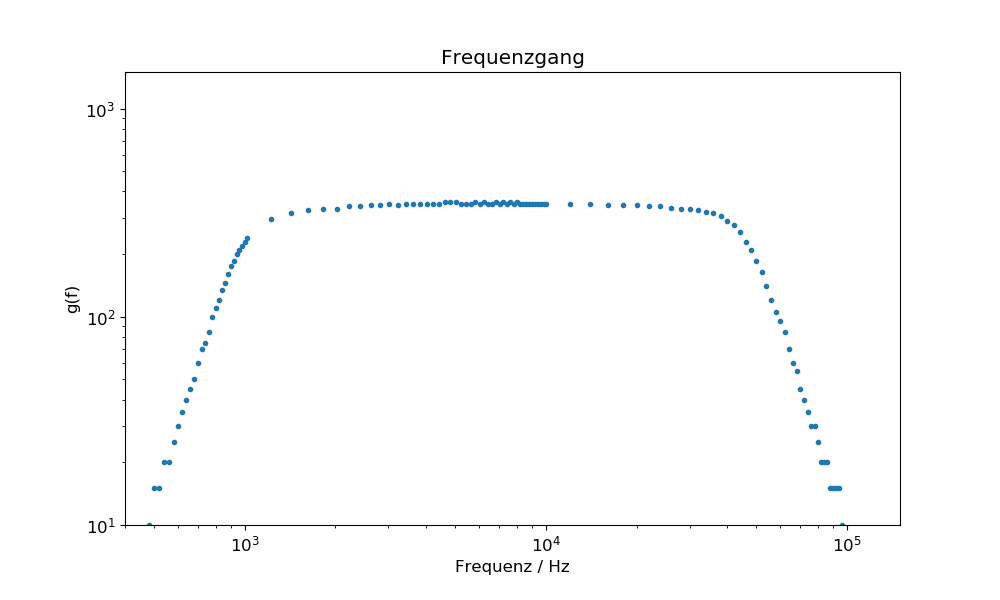
\includegraphics[width=.8\textwidth]{files/freq_data.png}
  \caption{Frequenzgang $g(f)$ bei konstanter Eingangsspannung und kontinuierlicher Frequenz}
  \label{plot:frequenzgang}
\end{figure}

Wir auch dem angefügten Python-Skript zu entnehmen, betrachten wir einen bereinigten Bereich des Frequenzgangs, ohne ein- und auslaufende Werte. 

Die zu fittende Funktion ist gegeben durch
\begin{align}
  g(f) = \frac{V}{\sqrt{1 + \flatfrac{1}{(\flatfrac{f}{\Omega_1})^{2 n_1}}} \sqrt{1 + (\flatfrac{f}{\Omega_2})^{2 n_2}}}.
\end{align}
Diese beschreibt den Frequenzgang einer Hintereinanderschaltung eines Verstärkers, eines Hochpassfilters der Ordnung $n_1$ mit Grenzfrequenz $\Omega_1$, sowie eines Tiefpassfilters der Ordnung $n_2$ mit Grenzfrequenz $\Omega_2$. Als Startparameter für den Fit wählen wir
\begin{table}[H]
  \centering
  \begin{tabular}{l|l}
    Variable & Startwert\\\hline
    Verstärkung $V$ & 1000\\
    Untere Grenzfrequenz $\Omega_1$ & 1000\\
    Obere Grenzfrequenz $\Omega_2$ & 50000\\
    Filterordnung $n_1, n_2$ & 5
  \end{tabular}
  \caption{Startwerte für \texttt{curve\_fit} der Daten an $g(f)$}
  \label{tab:startparams_fitfreq}
\end{table}

Abbildung \ref{plot:frequenzgang_fit} zeigt das Resultat des Fits. Die genauen Werte der optimierten Parameter sind an dieser Stelle der Übersichtlichkeit halber nicht angegeben, können aber dem angehängten Python Code entnommen werden.

\begin{figure}[H]
  \centering
  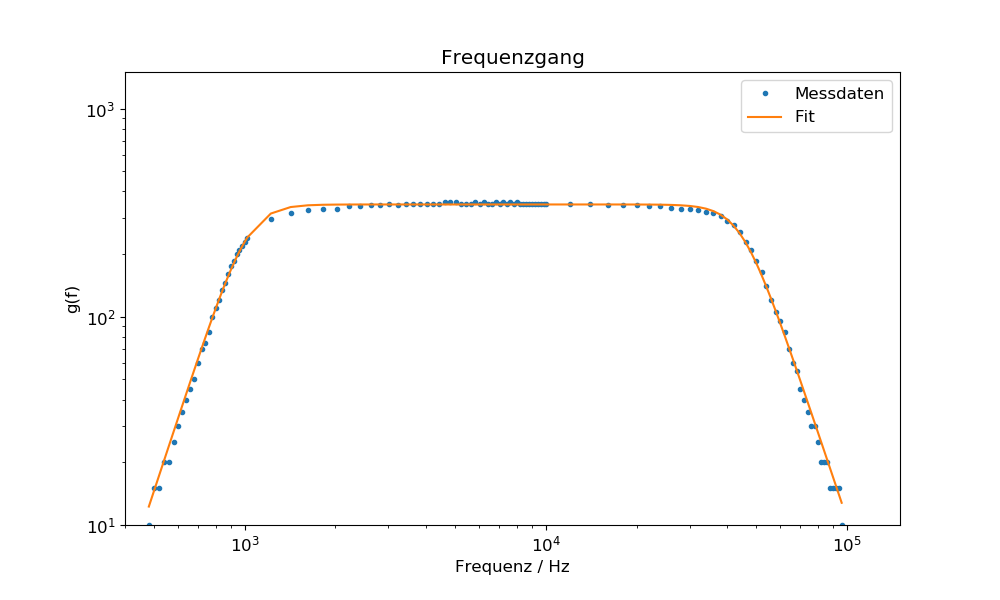
\includegraphics[width=.8\textwidth]{files/freq_data_fit.png}
  \caption{Frequenzgang $g(f)$ mit Fit}
  \label{plot:frequenzgang_fit}
\end{figure}

% \begin{table}[H]
%   \centering
%   \begin{tabular}{l|l}
%     Variable & Wert\\\hline
%     Verstärkung $V$ & $346.5 \pm 0.9$\\
%     Untere Grenzfrequenz $\Omega_1$ & $1027.9 \pm 4.8$\\
%     Obere Grenzfrequenz $\Omega_2$ & $44598.4 \pm 203.8$\\
%     Filterordnung $n_1$ & $4.39 \pm 0.10$\\
%     Filterordnung $n_2$ & $4.30 \pm 0.09$\\
%   \end{tabular}
%   \caption{Optimierte Paramter}
%   \label{tab:freq_fitted_params}
% \end{table}

Um die Rauschbandbreite zu bestimmen, quadrieren wir zunächst die Funktion $g(f)$ und integrieren das Ergebnis numerisch im zuvor festgelegten Wertebereich der Frequenz. Die Integration liefert uns einen Wert von
\begin{align}
  B = (5.35 \pm 0.11) \cdot 10^9 \si{\hertz}.
\end{align}
Der Fehler von $B$ ist rein systematischer Natur und setzt sich aus unterschiedlichen Faktoren, wie Untergrund, Genauigkeit der Messinstrumente und auch Integrationsfehler zusammen. Zusammenfassend wählen wir daraus für die Größe einen relativen Fehler von $2\%$, wie es auch in der Praktikumsanleitung angegeben ist. Mit diesem Wert fahren wir zum nächsten Schritt fort.

\subsection{Bestimmung der Boltzmannkostante}

Für die Bestimmung der Boltzmannkonstante erinnern wir uns zunächst an die Nyquist-Beziehung
\begin{align}
  \mean{U_r^2} = 4kTR\Delta f
\end{align}
für den Effektivwert der Rauschspannung $U_r$. Ersetzen wir die Bandbreite $\Delta f$ durch die zuvor bestimmte Rauschbandbreite $B$, so ergibt sich ein linearer Zusammenhang zwischen dem Widerstand $R$ und $\mean{U_r^2}$ mit Steigung 
\begin{align}
  c = 4 k T B. \label{eq:slope_rms}
\end{align}

Um diese Steigung zu bestimmen, ziehen wir nun die Daten, aufgenommen in Aufgabenteil 2, hinzu. In Plot \ref{plot:Ur_daten} zu sehen sind für die jeweiligen Widerstände die gemessenen Rauschspannungen $U_r$ abzüglich der Rauschspannung der Messelektronik $U_V$, jeweils quadriert.

\begin{figure}[H]
  \centering
  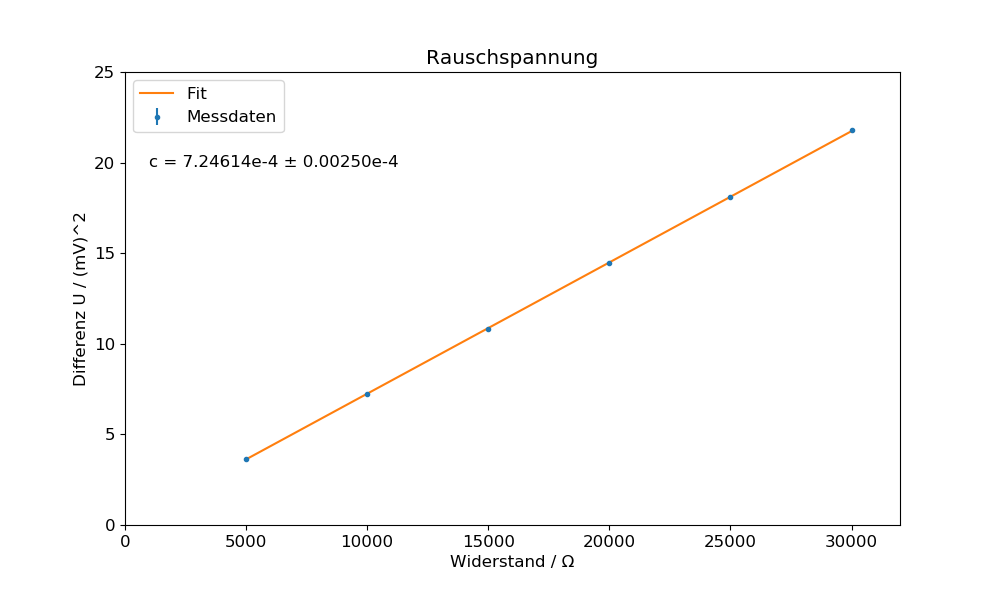
\includegraphics[width=.8\textwidth]{files/ur_data_fit.png}
  \caption{Rauschspannung der Widerstände abzüglich der Rauschspannung der Messelektronik}
  \label{plot:Ur_daten}
\end{figure}

An diese Daten fitten wir nun eine einfache lineare Funktion der Form $f(x) = cx$. Das Ergebnis des Fits ist bereits als Gerade in Abbildung \ref{plot:Ur_daten} zu sehen. Die bestimmte Steigung liegt bei
\begin{align}
  c = (7.2461 \pm 0.0026) \cdot 10^{-4} \si{\milli\volt\squared\per\ohm}.
\end{align}
%7.24614e-4 ± 0.00250e-4

Um zusätzlich die Güte des Fits zu untersuchen, betrachten wir nun einmal die $\chi^2$-Summe, sowie die reduzierte $\chi^2$-Summe, $\chi^2_\text{red}$.

\begin{align}
  \chi^2 &= 83.07\\
  \chi^2_\text{red} &= 16.61
\end{align}

Die Fitwahrscheinlichkeit für eine Wiederholungsmessung berechnete sich zu einem Wert von $0.0$\%.

Durch Umstellen der Gleichung (\ref{eq:slope_rms}) erhalten wir eine Formel für die Boltzmannkonstante
\begin{align}
  k = \frac{c}{4 T B}. \label{eq:boltzmann}
\end{align}

Die bis jetzt in der Auswertung nicht erwähnte Umgebungstemperatur $T$ ist ebenfalls dem Messprotokoll zu entnehmen. Diese lag bei $T = (23.00 \pm 0.10) \si{\degreeCelsius}= (296.15 \pm 0.10) \si{\kelvin}$.

Setzen wir nun alle Werte in (\ref{eq:boltzmann}) ein so erhalten wir für die Boltzmannkonstante einen Wert von 
\begin{align}
  k = (11.435 \pm 0.004\, \text{(stat.)} \pm 0.229\, \text{(sys.)}) \cdot 10^{-23} \si{\joule\per\kelvin}.
\end{align}

Wie der Praktikumsanleitung zu entnehmen, entspricht der statistische Fehler von $k$ gerade dem relativen Fehler von $c$;
\begin{align}
  \Delta k_{\text{stat.}} = \frac{\Delta c}{c} k.
\end{align}

Der systematische Fehler setzt sich zusammen aus dem Fehler der Zimmertemperatur $T$, sowie dem Fehler von $B$. Letzterer ist als eine Zusammensetzung verschiedener systematischer Fehlerquellen auf $\flatfrac{\Delta B}{B} = 2 \%$ abgeschätzt;
\begin{align}
  \Delta k_{\text{sys.}} = \sqrt{\qty(\frac{\Delta T}{T})^2 + \qty(\frac{\Delta B}{B})^2} k.
\end{align}